\documentclass[conference]{IEEEtran}
\IEEEoverridecommandlockouts
% The preceding line is only needed to identify funding in the first footnote. If that is unneeded, please comment it out.
%Template version as of 6/27/2024

\usepackage{cite}
\usepackage{amsmath,amssymb,amsfonts}
\usepackage{algorithmic}
\usepackage{graphicx}
\usepackage{textcomp}
\usepackage{xcolor}
\usepackage{hyperref}
\def\BibTeX{{\rm B\kern-.05em{\sc i\kern-.025em b}\kern-.08em
    T\kern-.1667em\lower.7ex\hbox{E}\kern-.125emX}}
\begin{document}

\title{Steam Database: Analisis exploratorio y preprocesamiento
}

\author{\IEEEauthorblockN{1\textsuperscript{ro} David Felipe Marin Rosas}
  \IEEEauthorblockA{\textit{Facultad de Ingeniería} \\
    \textit{Universidad Nacional De Colombia}\\
    Bogotá, Colombia \\
    dmarinro@unal.edu.co}
  \and
  \IEEEauthorblockN{2\textsuperscript{do} Gian Emanuel Morales González}
  \IEEEauthorblockA{\textit{Facultad de Ingeniería} \\
    \textit{Universidad Nacional De Colombia}\\
    Bogotá, Colombia \\
    gimoralesg@unal.edu.co}
  \and
  \IEEEauthorblockN{3\textsuperscript{ro} Juan Felipe Bejarano Salazar}
  \IEEEauthorblockA{\textit{Facultad de Ingeniería} \\
    \textit{Universidad Nacional De Colombia}\\
    Bogotá, Colombia \\
    jbejaranos@unal.edu.co}
  \and
  \IEEEauthorblockN{4\textsuperscript{to} Luis Esteban León Rojas}
  \IEEEauthorblockA{\textit{Facultad de Ingeniería} \\
    \textit{Universidad Nacional De Colombia}\\
    Bogotá, Colombia \\
    luleonr@unal.edu.co}
}

\maketitle

\begin{abstract}
This document details the exploratory data analysis and preprocessing of the ``Steam Games Dataset'', which contains information from over 120,000 video games published on the Steam platform. The objective is to analyze its features (prices, concurrent players, reviews, genres) to build a clean and ready-to-use dataset for predictive models. Through visualizations and robust statistical measures, it was identified that the market exhibits a strong asymmetry: there is a vast number of low-impact free games compared to a small number of massive hits. These findings guided the data cleaning process, null value handling, and feature engineering, setting the groundwork to predict the commercial success of future video games in a structured manner.
\end{abstract}

\begin{IEEEkeywords}
  videojuegos, análisis exploratorio, preprocesamiento, steam database, python, pandas, matplotlib, seaborn, patrones de compra, tendencias de juego, comportamiento del consumidor
\end{IEEEkeywords}

\section{Introducción}

En la última década, la industria de los videojuegos ha experimentado un crecimiento exponencial, consolidándose como uno de los sectores de entretenimiento más lucrativos a nivel global. Dentro de este ecosistema, Steam, operada por Valve Corporation, se mantiene como la plataforma de distribución digital dominante para PC. Con miles de títulos lanzados anualmente, la plataforma genera un volumen masivo de datos que reflejan tendencias de consumo, estrategias de precios y preferencias de género.

El presente documento se centra en el estudio del "Steam Games Dataset", una recopilación de datos a partir de la API ofrecida por steam. Este conjunto de datos captura la diversidad del catálogo de Steam, permitiendo observar desde grandes producciones AAA hasta el emergente mercado de juegos independientes (Indie).

\section{Objetivo}


Analizar qué variables del conjunto de datos influyen más en el éxito de un videojuego. Para este estudio, nuestras tres variables esenciales y métricas de éxito serán: el porcentaje de reseñas positivas categorizado (indicando cantidad total y la razón de aprobación), el número de ventas (\textit{Estimated owners}), y la cantidad de jugadores simultáneos (\textit{Peak CCU}). Con esto, se busca sentar las bases para crear modelos predictivos que estimen el éxito comercial de futuros desarrollos y descubrir qué características se necesitan para triunfar dentro de nichos específicos de mercado.

\section{Descripción del conjunto de datos}
Se utilizó el ``Steam Games Dataset'' \cite{steamDataset}, obtenido a partir de la API oficial de Steam. Este \textit{dataset} cuenta con 122\,611 registros, correspondientes cada uno a un videojuego único, y está compuesto por 39 variables originales.

Las variables abarcan diferentes tipos (ver Figura \ref{fig:dist_vars}): nominales absolutas como el identificador (\textit{AppID}) y nombre (\textit{Name}); de razón para características continuas como el precio (\textit{Price}) y la máxima cantidad de jugadores simultáneos (\textit{Peak CCU}); ordinales como la estimación de compradores (\textit{Estimated owners}); y variables con múltiples valores nominales, como los géneros (\textit{Genres}) y categorías (\textit{Categories}).

\begin{figure}[htbp]
  \centerline{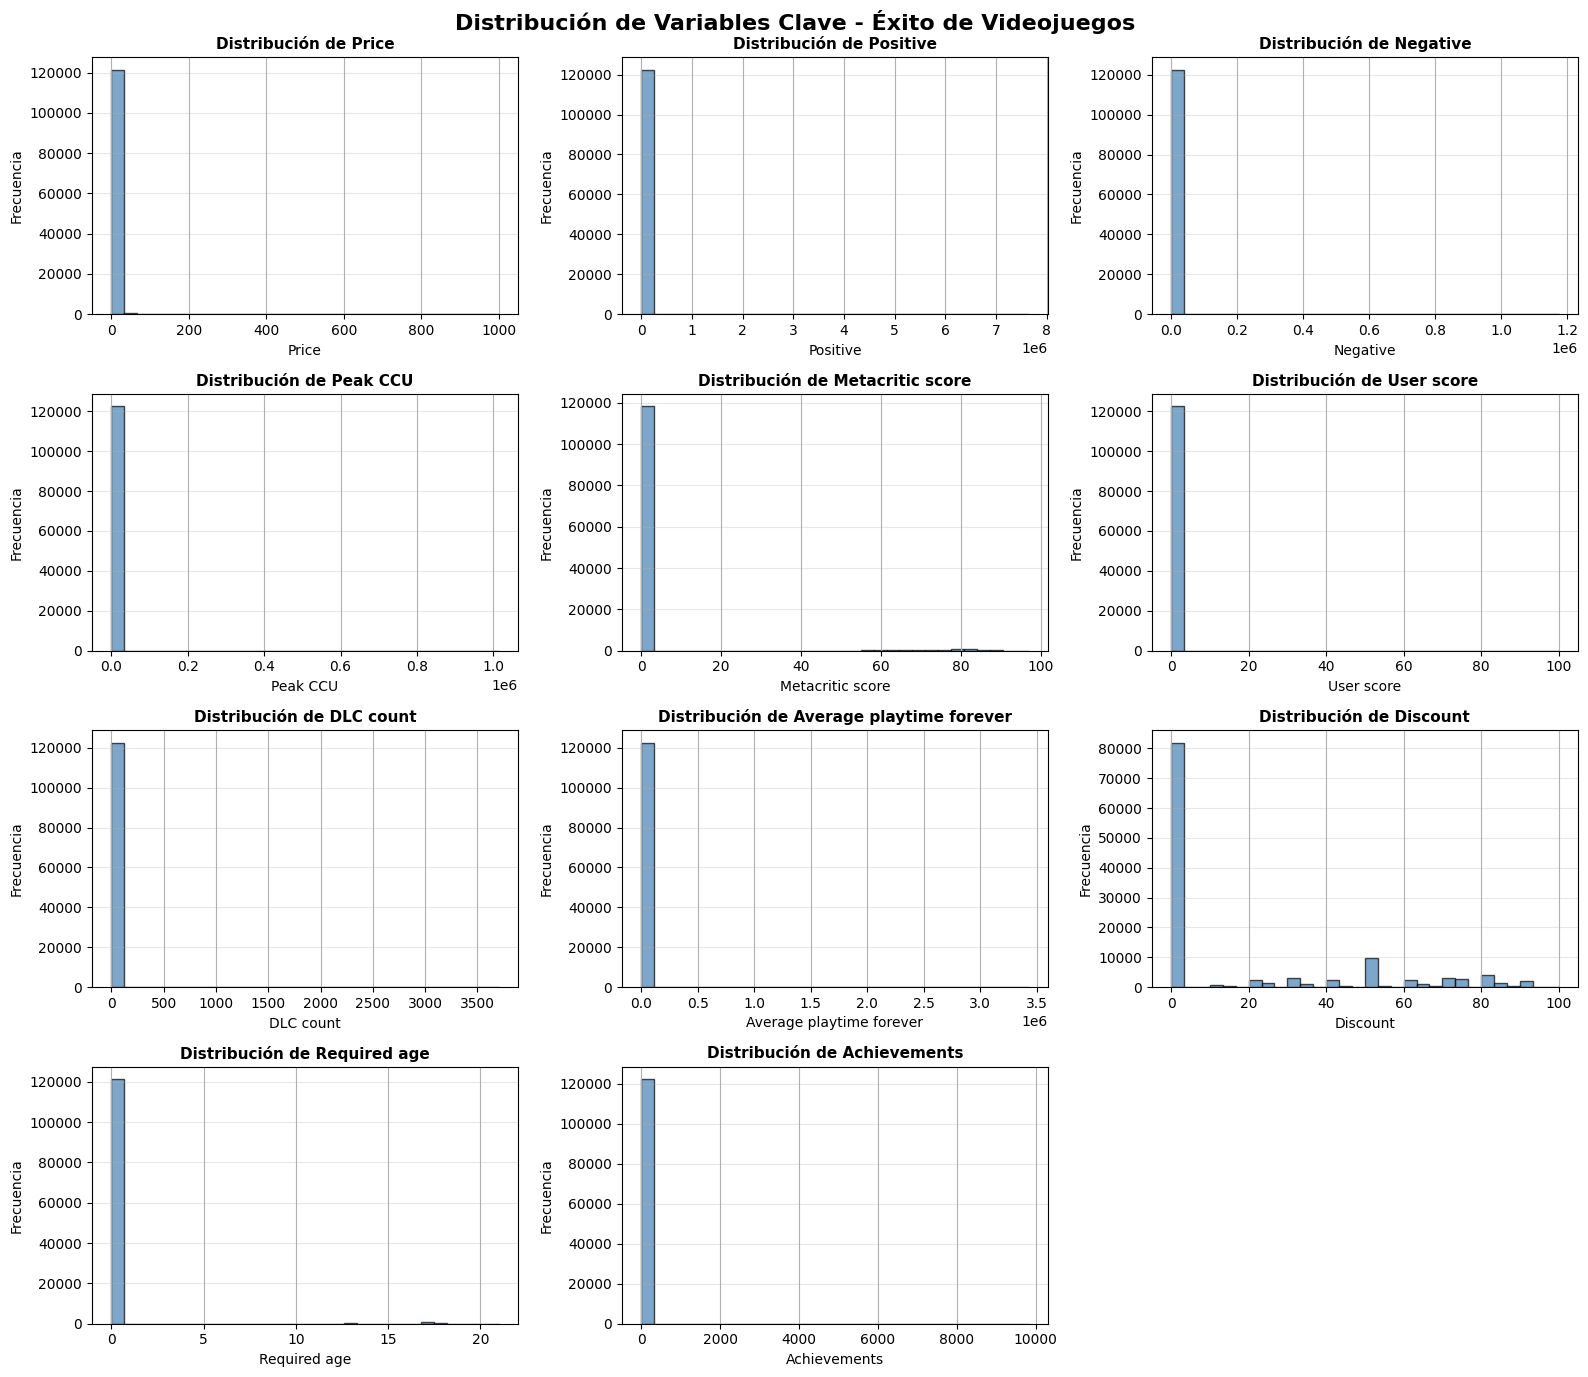
\includegraphics[width=\linewidth]{figures/grafica_1.png}}
  \caption{Distribución de frecuencias para las variables numéricas de Steam. Se evidencia una gran asimetría hacia el lado izquierdo.}
  \label{fig:dist_vars}
\end{figure}

\section{Análisis Exploratorio y Resultados}

\subsection{Análisis de Frecuencias y Medidas de Centralidad}
En la exploración inicial, se observó que casi todos los juegos son compatibles con Windows, superando ampliamente a los desarrollos para Mac y Linux. Al revisar variables numéricas como el precio y el máximo de jugadores activos (\textit{Peak CCU}), se evidenció que una porción muy pequeña de títulos acumula la gran mayoría de las cifras. Al existir tantos valores en cero o muy bajos, existe una enorme diferencia entre el promedio (media aritmética) y la mediana. Para mitigar el efecto de estos valores atípicos (\textit{outliers}), se calculó la \textbf{media truncada} (\textit{trimmed mean}), eliminando el 10\% de los datos más extremos de cada lado para obtener el comportamiento de un juego más ``típico''.

\begin{figure}[htbp]
  \centerline{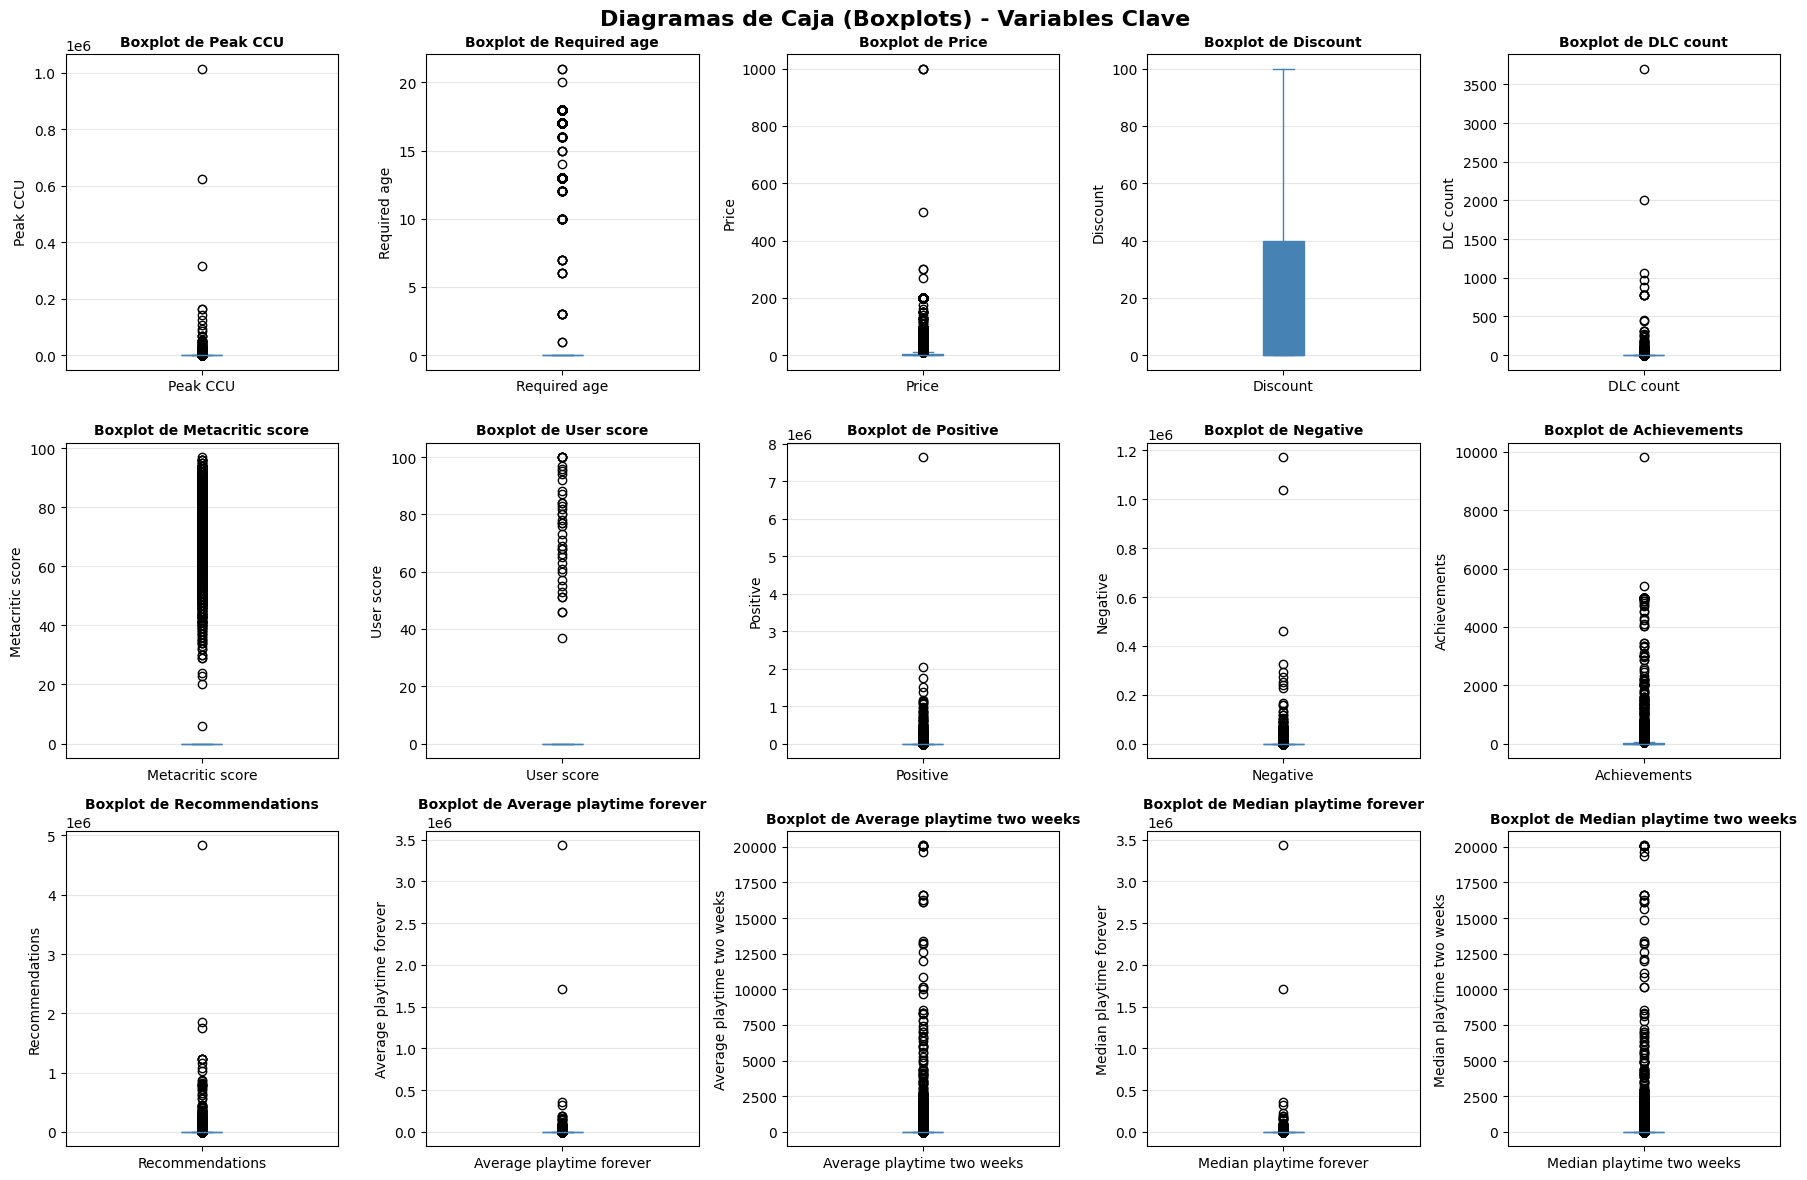
\includegraphics[width=\linewidth]{figures/grafica_5.png}}
  \caption{Diagramas de caja (\textit{Boxplots}) que muestran la gran cantidad de valores atípicos y la enorme dispersión generada por juegos sumamente populares.}
  \label{fig:boxplots}
\end{figure}

\subsection{Medidas de Dispersión y Distribuciones}
Para medir correctamente la dispersión de los datos sin afectar la precisión matemática a causa de de los valores atípicos, se priorizó la \textbf{Desviación Media Absoluta (AAD)}. Como se observa en la estimación de densidad KDE y en los diagramas de caja (Figura \ref{fig:boxplots}), atributos monetarios y de popularidad tienen una distribución marcadamente inclinada hacia la cota inferior. El mercado comercial se compone de innumerables títulos de bajo costo o completamente gratuitos con muy poco impacto, que contrastan fuertemente frente a las grandes y escasas franquicias \textit{AAA} o juegos virales.

\subsection{Causalidad Multivariada}
Al utilizar medidas de correlación lineal (coeficiente de Pearson), se encontraron relaciones claras y fundamentales. Por ejemplo, existe una fuerte asociación directa entre la máxima cifra récord de jugadores (\textit{Peak CCU}) y el volumen histórico de reseñas obtenidas (tanto positivas como negativas). Estos factores crecen directamente de acuerdo al volumen total de jugadores que atrae el título.

\section{Preprocesamiento de Datos}
Para asegurar que los datos del catálogo resulten óptimos para su uso en la fase de modelamiento algorítmico estadístico, se ejecutó un proceso riguroso de limpieza:

\subsection{Selección y Eliminación de Atributos}
Se descartaron todas las variables que no aportaban métricas relevantes para clasificar o predecir el éxito de un juego, tales como hipervínculos web, direcciones de correo de soporte y referencias multimedia promocionales (\textit{Header image}, \textit{Movies}, \textit{Screenshots}). Adicionalmente, se eliminaron columnas que se encontraban casi completamente vacías o rellenas de valores en cero, como \textit{User score} o \textit{Required age}, ya que estas interferían con la integridad de los modelos predictivos.

\begin{figure}[htbp]
  \centerline{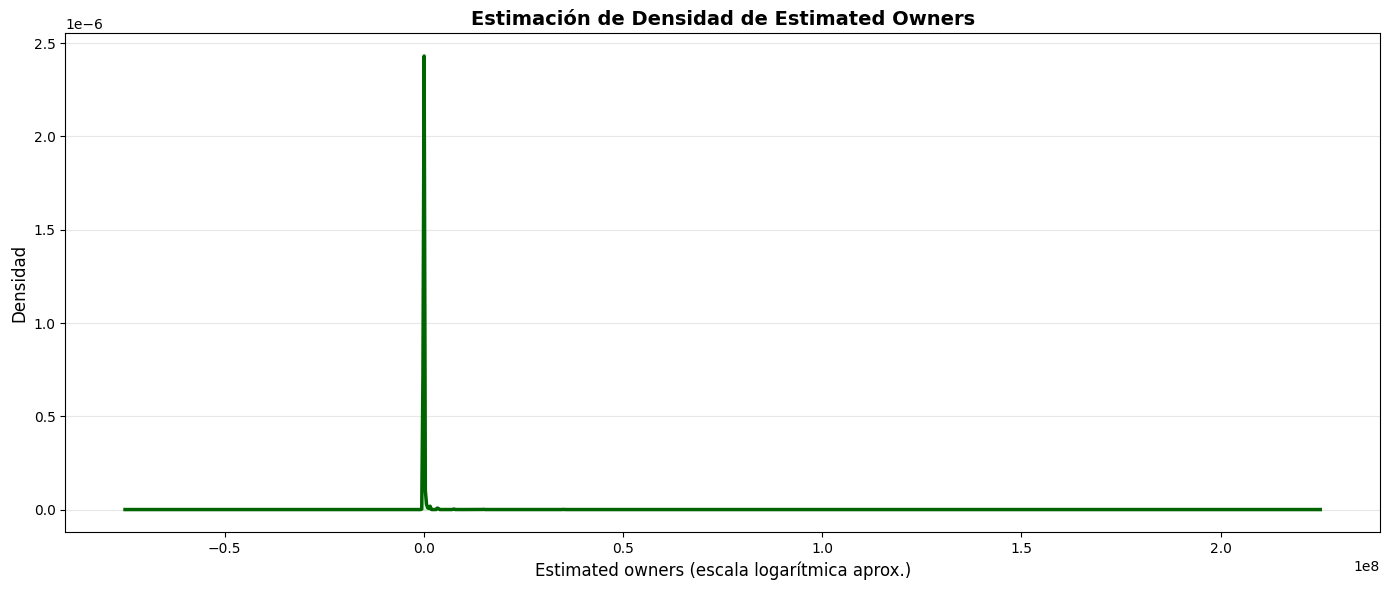
\includegraphics[width=\linewidth]{figures/grafica_4.png}}
  \caption{Estimación de densidad (KDE) para visibilizar las frecuencias en los rangos discretos de la cantidad estimada de jugadores (\textit{Estimated Owners}).}
  \label{fig:kde_owners}
\end{figure}

\subsection{Tratamiento de Valores Faltantes (Nulos)}
A través de la inspección sobre la ausencia de datos, se identificó que no figurar con un autor y empresa encargada (\textit{Developer}) es comúnmente una señal relacionada a estafas o desarrollos falsos subidos a la red de Steam; por este motivo, se purgaron completamente las filas que carecían de dicho identificador. Por el contrario, es un comportamiento normal que las variables categóricas o descriptivas queden en blanco (ej. \textit{Genres}, \textit{Tags}, \textit{Publishers}) debido a la forma de registro de algunos títulos. Estos casos orgánicos ausentes fueron cubiertos sistemáticamente con el identificador de texto ``NA'' para evitar corrupciones estructuradas. Toda métrica unívocamente matemática registró niveles completos, por lo que no existieron vacíos numéricos que imputar.

\subsection{Ingeniería de Atributos y Discretización}
El preprocesamiento del precio exhibía un desafío dada la enorme recurrencia de valores nominales fijados en \$0.00. Para contrarrestarlo, la cifra escalar \textit{Price} fue extraída bajo bandas de clasificación ordinales (\textit{Price\_category}), replicando las barreras comerciales comúnmente encontradas entre consumidores (juegos gratuitos, juegos muy baratos, o el tope tradicional de \$59.99). De igual forma lógica, la cadena textual correspondiente a la fecha de publicación (\textit{Release date}) se separó minuciosamente en tres diferentes campos tabulares: año, mes, y estación de lanzamiento. Esto habilitará la futura extracción estacional de picos de consumo anual.

\subsection{Manejo Condicional de Valores Atípicos}
La estrategia para atenuar valores atípicos se dictaminó con el algoritmo clásico del rango intercuartílico (IQR). En el campo preciso de los análisis tarifarios, se evidenció que aislar en dos sub-estratos independientes a los títulos ``Gratuitos'' en relación a aquellos de ``Pago'', provocaba un impacto determinante para comprender o fijar el límite estadístico a partir de cuándo un valor era realmente un costo sumamente atípico. Referente a medidas de popularidad de éxito irruptivo tales como la congregación máxima histórica (\textit{Peak CCU}), se optó intencionalmente por conservar intactos todos sus datos hiper-extendidos. Esto obedece a que limitar arbitrariamente dichos volúmenes resultaría en amputar a los protagonistas absolutos y al concepto fundamental del ``éxito'', mermando completamente las proyecciones algorítmicas hacia los verdaderos gigantes del mercado de videojuegos.


\subsection{Transformaciones Orientadas al Modelamiento}
Dependiendo de los análisis específicos que se deseen realizar en etapas posteriores, se deberá procesar aún más ciertas características. Por ejemplo, para analizar los títulos mejor calificados, se utilizará la variable creada a partir de las reseñas para descartar, de manera acorde al algoritmo de recomendación de Steam, aquellos juegos que tengan calificaciones de ``Mayormente Positivas'' (\textit{Mostly Positive}) o inferiores. Por otro lado, para variables de cardinalidad múltiple, como las categorías y los géneros, será necesario crear una variable con valores booleanos por cada género individual (\textit{One-Hot Encoding}), facilitando así su uso matemático en los modelos de datos.

\section{Conclusión y Trabajos Futuros}
El trabajo de minería descriptiva y preprocesamiento de datos permite establecer una verdad fundamental sobre la industria digital lúdica: las plataformas dominantes de distribución como Steam no actúan bajo condiciones equilibradas u homogéneas. Este mercado es netamente asimétrico y se caracteriza por una gigantesca e invisible aglomeración de micro-proyectos amater o títulos gratuitos con actividad mínima, la cual constrasta bruscamente contra un pequeñísimo grupo cerrado de obras monumentales mundiales. Por esta precisa causalidad, las técnicas de depuración simplistas son inviables. Comprobó ser un requerimiento inexcusable el clasificar pormenorizadamente los horizontes temporales de ventas, separar bajo un vector exclusivo a aquellas producciones dependientes de cero ingresos, y metodológicamente, salvaguardar y retener con fiereza y convicción a los atípicos hiper-dimensionados en popularidad para comprender eficientemente un modelo veraz a futuro. En definitiva, las transformaciones estandarizadas ejecutadas dotan al \textit{Steam Games Dataset} con robustez matricial plena para acoplarse con altísimo desempeño en las ulteriores etapas algorítmicas de inteligencia de máquina previstas para este proyecto investigativo.







\nocite{*}
\bibliographystyle{IEEEtran}
\bibliography{ref}



\end{document}
